%/////////////////////////////////////////////////////////%
%//						PREAMBLE						//%
%/////////////////////////////////////////////////////////%

\documentclass[11pt]{report}

%%%%%%%%%%%%%%%%%%%%%%%
% 	  Packages
%%%%%%%%%%%%%%%%%%%%%%%

%% Fonts and Symbols
%% --------------------------
\usepackage{
			amsmath,			% math operators
			amssymb,			% math symbols
			}

%% Graphics
%% --------------------
\usepackage[pdftex,dvipsnames]{xcolor}  % Coloured text etc.
\usepackage{
			graphicx,			% allows insertion of images
			subfigure,			% allows subfigures (a), (b), etc.
			}
\graphicspath{ {graphics/} }	% (graphicx) relative path to graphics folder

%% Tables
%% --------------------------
\usepackage{
			booktabs,			% better tables, discourages vertical rulings
			multicol,			% allow multi columns
      multirow,     % allow multi rows
			}

%% Layout Alteration
%% --------------------------
\usepackage{
			enumitem,			% indented items for glossary
			framed,				% nice boxes; used in Supervisor's Approval
			geometry,			% change the margins for specific PAGES
			}
\setlist[description]{style=nextline}
\geometry{						% specify page size options for (geometry)
			a4paper, 			% paper size
			margin=1in,			% specified independently with hmargin vmargin
		 }

%% Units
%% --------------------------
\usepackage{
			siunitx,			% has S (decimal align) column type
			}
\sisetup{input-symbols = { () },  % do not treat "(" and ")" in any special way
         group-digits  = false, % no grouping of digits
%		 load-configurations = abbreviations,
%		 per-mode = symbol,
		 }

%% Misc
%% --------------------------
\usepackage{
			pdfpages,			% import pdfs into this document -- used for the Letter
			url,				% allows urls to be added to document
      xargs,      % more than one optional arg in new commands
			}
% preserve default font for URLs
\renewcommand*{\UrlFont}{\rmfamily}
% todo notes setup
\usepackage[colorinlistoftodos,prependcaption,textsize=small]{todonotes}

%% Bibliography
%% --------------------------
\usepackage[
	backend=biber,
	style=ieee]
{biblatex}
\addbibresource{final.bib}


%%%%%%%%%%%%%%%%%%%%%%%
% 	Environments
%%%%%%%%%%%%%%%%%%%%%%%
% Hides the formatting for the summary
\newenvironment{Overview}
	{ % beginning formatting
		% manually add entry to the toc since section*
		% suppresses addition to toc
		\addcontentsline{toc}{chapter}{Overview}
		\topskip0pt				% remove top padding
		\vspace*{\stretch{2}}	% Pad 2/3 of the page length
		\chapter*{Overview}		% don't append a chapter num before "Overview"
	}
	{ % end formatting
		\vspace*{\stretch{3}}
	}


%%%%%%%%%%%%%%%%%%%%%%%
% Macros and Commands
%%%%%%%%%%%%%%%%%%%%%%%

% todo note styles
\newcommandx{\stub}[1]{\todo[linecolor=OliveGreen,backgroundcolor=OliveGreen!25,bordercolor=OliveGreen,inline=true]{#1}}
\newcommandx{\maybe}[1]{\todo[linecolor=blue,backgroundcolor=blue!25,bordercolor=blue,inline=true]{#1}}
\newcommandx{\improvement}[2][1=]{\todo[linecolor=Plum,backgroundcolor=Plum!25,bordercolor=Plum,#1]{#2}}
\newcommand{\citeneeded}{\todo[linecolor=red,backgroundcolor=red!25,bordercolor=red]{cite needed}}
\newcommandx{\thiswillnotshow}[2][1=]{\todo[disable,#1]{#2}} % demo: add 'disable' to note types

% override S column type with centered text column
\providecommand{\textcol}[1]{\multicolumn{1}{c}{#1}}

% provides a place to write on documents; like __________________ that
\providecommand{\blankline}[1]{\rule{#1}{0.5pt}}

% Set up page numbering for appendices as (Appendix Letter) - (Page Number)
\providecommand{\StartAppendices}{
    \newpage
    \newcounter{AppendixCounter}
    \renewcommand{\thepage}{\Alph{AppendixCounter} \textendash\ \arabic{page}}
}

% Manually construct the section title for each appendix and then
% add an entry to the ToC
\providecommand{\Appendix}[1]{
    \newpage
    \stepcounter{AppendixCounter}
    \setcounter{page}{1}
    \section*{Appendix \Alph{AppendixCounter}\quad #1}
    \addtocontents{toc}{\protect\contentsline{chapter}%
    	{Appendix \Alph{AppendixCounter}\quad #1}{}}
	% \protect preserves the spacing in the ToC
}

% Blank lines for marks on the title page
\providecommand{\markline}{\rule{1cm}{0.5pt}}

%/////////////////////////////////////////////////////////%
%//						BODY							//%
%/////////////////////////////////////////////////////////%

\begin{document}

%%%%%%%%%%%%%%%%%%%%%%%
% 	  Title Page
%%%%%%%%%%%%%%%%%%%%%%%
\pagenumbering{gobble}		% turn off page numbering
\begin{titlepage}

  \begin{center}
    \begin{LARGE}
      Department of Electrical and Computer Engineering \\
      University of Victoria \\
      SENG 462 \textemdash{} Distributed Systems and the Internet \\[1cm]
      \textsc{Project Report}
      \\[1in]
    \end{LARGE}
  \end{center}

  \begin{tabular}{ p{0.25\textwidth} p{0.75\textwidth} }
    Report submitted on:& 11 April, 2017 \\
    To: & Prof.\ S.\ Neville \\
    & \\
    Names: & J.\ Cooper (V00794804)\\
    & T.\ Stephen (V00812021)\\
    & J.\ Vlieg (V00779758)\\[1in]
  \end{tabular}

  \begin{center}
    \begin{tabular}{rl}
      Architecture and project plan & \markline{} /5 \\
      Security & \markline{} /5 \\
      Test plan & \markline{} /5 \\
      Fault tolerance & \markline{} /5 \\
      Performance analysis & \markline{} /5 \\
      Capacity planning & \markline{} /5 \\
      & \\
      \textbf{Total} & \markline{} \textbf{/30} \\
    \end{tabular}
  \end{center}

\end{titlepage}


%%%%%%%%%%%%%%%%%%%%%%%
%    Front matter
%%%%%%%%%%%%%%%%%%%%%%%
\newpage
\addtocontents{toc}{~\hfill\textbf{Page}\par}	% 'Page' above the page numbers
\tableofcontents

\newpage
\pagenumbering{roman}	% i, ii, iii, ... page numbering
\addcontentsline{toc}{chapter}{\listfigurename}	% manually add to toc
\addtocontents{lof}{~\hfill\textbf{Page}\par}
\listoffigures

\newpage				% LoF and LoT may be on the same page if they fit
\addcontentsline{toc}{chapter}{\listtablename}
\addtocontents{lot}{~\hfill\textbf{Page}\par}
\listoftables

\begin{Overview}

The goal of the project was to build a distributed day trading system, with a focus on performance. The client original stated the following actions as business requirements:

\begin{itemize}
  \item View their account
  \item Add money to their account
  \item Get a stock Quote
  \item Buy a number of shares in a stock
  \item Sell a number of shares in a stock they own
  \item Set an automated sell point for a stock
  \item Set a automated but point for a stock
  \item Review their complete list of transactions
  \item Cancel a specified transaction prior to its being committed
  \item Commit a transaction
\end{itemize} 

Additionally, the overall architectural goals of the system were:
\begin{itemize}
  \item Minimum transaction processing times. 
  \item Full support for required features. 
  \item Reliability and maintainability of the system. 
  \item High availability and fault recoverability (i.e. proper use of fault tolerance) 
  \item Minimal costs (development, hardware, maintenance, etc.) 
  \item Clean design that is easily understandable and maintainable. 
  \item Appropriate security 
  \item A clean web-client interface. 
\end{itemize}

These requirements form the basis for the distributed daytrading system commissioned by DayTrading Inc.

During the three month development period we created a distributed system capable of operating at over 26\,000 TPS.
We identified and corrected performance bottlenecks in the quote retrieval method and persistent audit log generation.
Current analysis indicates that total TPS will scale linearly with the number of workers, however the total throughput of the system is limited by the method for distributing transactions within the system.


We were able to accomplish all of the business and technical requirements laid out by DayTrading Inc, as well as our personal objectives for the system. We built an event based system utilizing the frameworks, tools, and language that we originally planned. Slight modification of the system occurred throughout the design process, but in general the planned architecture stayed relatively the same throughout the entire implementation. Golang proved to be an excellent choice for the system based on its speed, ease of user, and idiomatic patterns which lined up extremely well with an event sourcing framework like RabbitMQ. Rabbit and Redis also worked extremely well, and proved to be both fast and durable when it came to transactions per second and fault tolerance. Websockets proved to be a great way to send the event sourced data back to the frontend, since websockets is again an event sourced pattern for web communications. While relatively simple to setup, the handshaking and setting up of the socket hub proved to be a little bit complex to sort out. The original handshake system functioned for basic testing, but when simulated over multiple users, the socket hub would crash. The addition of mutexes solved this issue without much drain on performance for socket initialization and tracking.

Testing was performed with a combination of manual and automated testing, along with continuous integration testing, unit testing critical components, and manual testing of business logic and SLA compliance. This proved to be an effective method for ensuring code quality.  Further automated unit testing, integration testing, and  regression testing would likely have cut down on development time, the strategy used proved to be adequate for the needs.  The inclusion of the RabbitMQ management console, a fake quote server, and a comprehensive logging repository proved to drastically simplify and streamline the manual testing process, and proved to meet the needs of the developers.

The systems fault tolerant behavior is derived from its event sourcing pattern. By auditing logging the system, we are able to keep track of which events should exist on which worker, and if a worker is to go down, we can replay those events back onto a new or existing instance, recovering the complete user state of the account. A variety of other fault tolerant measures were implemented, including compile time type safety to minimize runtime errors.

A variety of security features were implemented to protect the user's information and the system’s functionality. Post requests for actions are sanitized to ensure that only correct commands will make it into Redis, and are then again checked when they leave Redis to be consumed by the worker. We also maintain a layer of random security by never revealing which worker the account exists on. If a user was to attack a worker, they could in theory try forever since the account may or may not exist on that instance.

Additional improvements to the system have been outlined, and could be implemented given more time for the project. While the deadline was reached with all requirements fulfilled, there is still much improving that could be done to the system to make it harder, better, faster, stronger.


\end{Overview}


%%%%%%%%%%%%%%%%%%%%%%%
%		Main Body
%%%%%%%%%%%%%%%%%%%%%%%
\newpage
\pagenumbering{arabic}	% 1, 2, 3, ... page numbering

\chapter{Performance analysis}

\section{Technology}

\subsection{Golang}
Golang was selected originally because it gives a lot of tools to maximize scalability, but is also very easy to learn and use efficiently.
Golang’s idioms are relatively easy to learn and the architectural decisions Rob Pike made when bringing the language to fruition heavily favor the task at hand.

Golang has extremely lightweight threading.
It is possible to spawn thousands of threads in a golang instance without bogging down a system.
New threads are made for goroutines, http request, etc, and are managed by the golang thread scheduler, not the OS.
This allows for a lot of multithreaded benefit without a lot of the multithreaded headache.
Golang goroutines and the producer/consumer model are very easily implemented.
We wanted to utilize a language which was able to:

\begin{itemize}
  \item Efficiently scale
  \item Work well with RMQ
  \item Be easy to learn and fun to use.
\end{itemize}

Golang fulfills all of these categories.
The idea of channels in golang is almost identical to the consumption of RabbitMQ channels, and was very easy to hook into the golang flow.

Golang has the added benefit of being both type safe, and well supported by the community.
The former makes it incredibly easy to debug and refactor code.
The latter means that there are a whole set of profiling and testing tools available by default, so we did not have to go out and research what the best ones were.

\subsection{RabbitMQ}
We selected RabbitMQ early on as we wanted to do an event based system, and wanted to be able to communicate between components effortlessly.
With an event based system, we wanted to utilize a communication protocol that would perform FIFO communication between microservices.
Rabbit fills this need exactly, and the documentation is verbose enough that ramp up time is minimal.
It is easily deployed with docker, and the management console is very easy to use and get a good picture of the system state.
It also offers the ability to inject messages directly into queues and exchanges, as well as many other testing features.

\subsection{Redis}
Redis is a distributed, in memory key-value store that supports publish-subscribe events.
We used Redis to provide caching for quotes, unhandled transactions and as a log message buffer.
We used key TTLs to enforce quote validity windows.
Although Redis operates as an in memory data store it writes changes to disk every sixty seconds in order to minimize data loss on system failure.

\subsection{Postgres}
Changes to user account state, retrieved quotes and user transactions are logged in a Postgres database for storage.
Postgres offers full ACID compliance which allows the database to act as a ``source of fact'' for recreating the historical state of accounts in the system.

\subsection{Websockets} 
Websockets allow asynchronous communication between the frontend and backend system components.
Data can be passed to a webpage without requiring a page reload or other user-triggered action.
This allows asynchronous events, like pending buy expirations or the fulfillment of a sell trigger, to be brought to the user's attention immediately.

\section{Original architecture}
\textit{Can steal most of this from the first report.}

\section{Technology}

\subsection{Golang}

\subsection{RabbitMQ}

\subsection{Redis}

\subsection{Postgres}

\subsection{Websockets}
\section{Work plan}
We held many meetings throughout the term on the subject of planning and task division. On average, we would meet once every week or two to modify design decisions and evolve the architecture. Whiteboarding of the design and architecture was documented.

\subsection{Timeline}
Cumulatively, we logged over 450 hours on this prototype. Figure~\ref{fig:work-per-week} shows the week-by-week breakdown. On average, we spent 38.125 hours building the prototype. 

\begin{figure}[tbph]
  \centering
  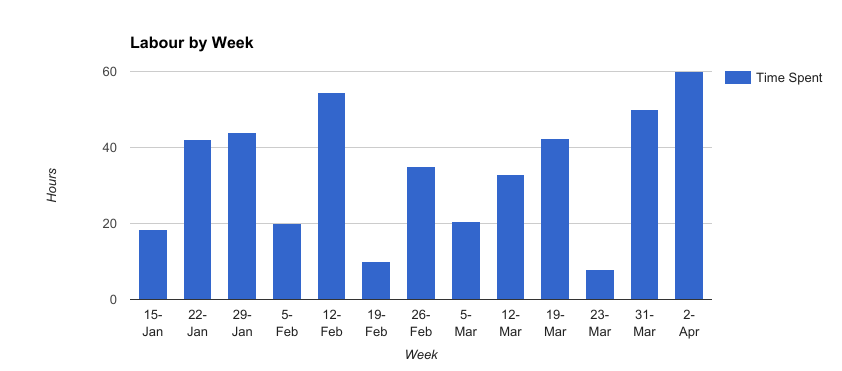
\includegraphics[width=0.85\linewidth]{graphics/work-per-week}
  \caption{Work per week on prototype, all tasks}
  \label{fig:work-per-week}
\end{figure}

Figure~\ref{fig:work-pie} shows that over half of the work time was spent on implementation. Design sessions took the form of collaborative whiteboarding and brainstorming activities with the group as a whole. 

\begin{figure}[tbph]
  \centering
  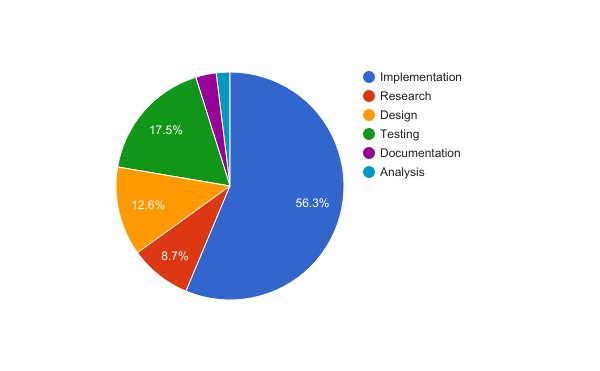
\includegraphics[width=0.7\linewidth]{graphics/work-pie}
  \caption{Areas of work}
  \label{fig:work-pie}
\end{figure}

System testing was almost exclusively through code review, where implementations were examined by other group members for output validity and code quality.



\section{Final architecture}
The final architecture, shown in Figure~\ref{fig:arch-final}, was as a whole relatively similar to our planned architecture. 

\begin{figure}[tbph]
  \centering
  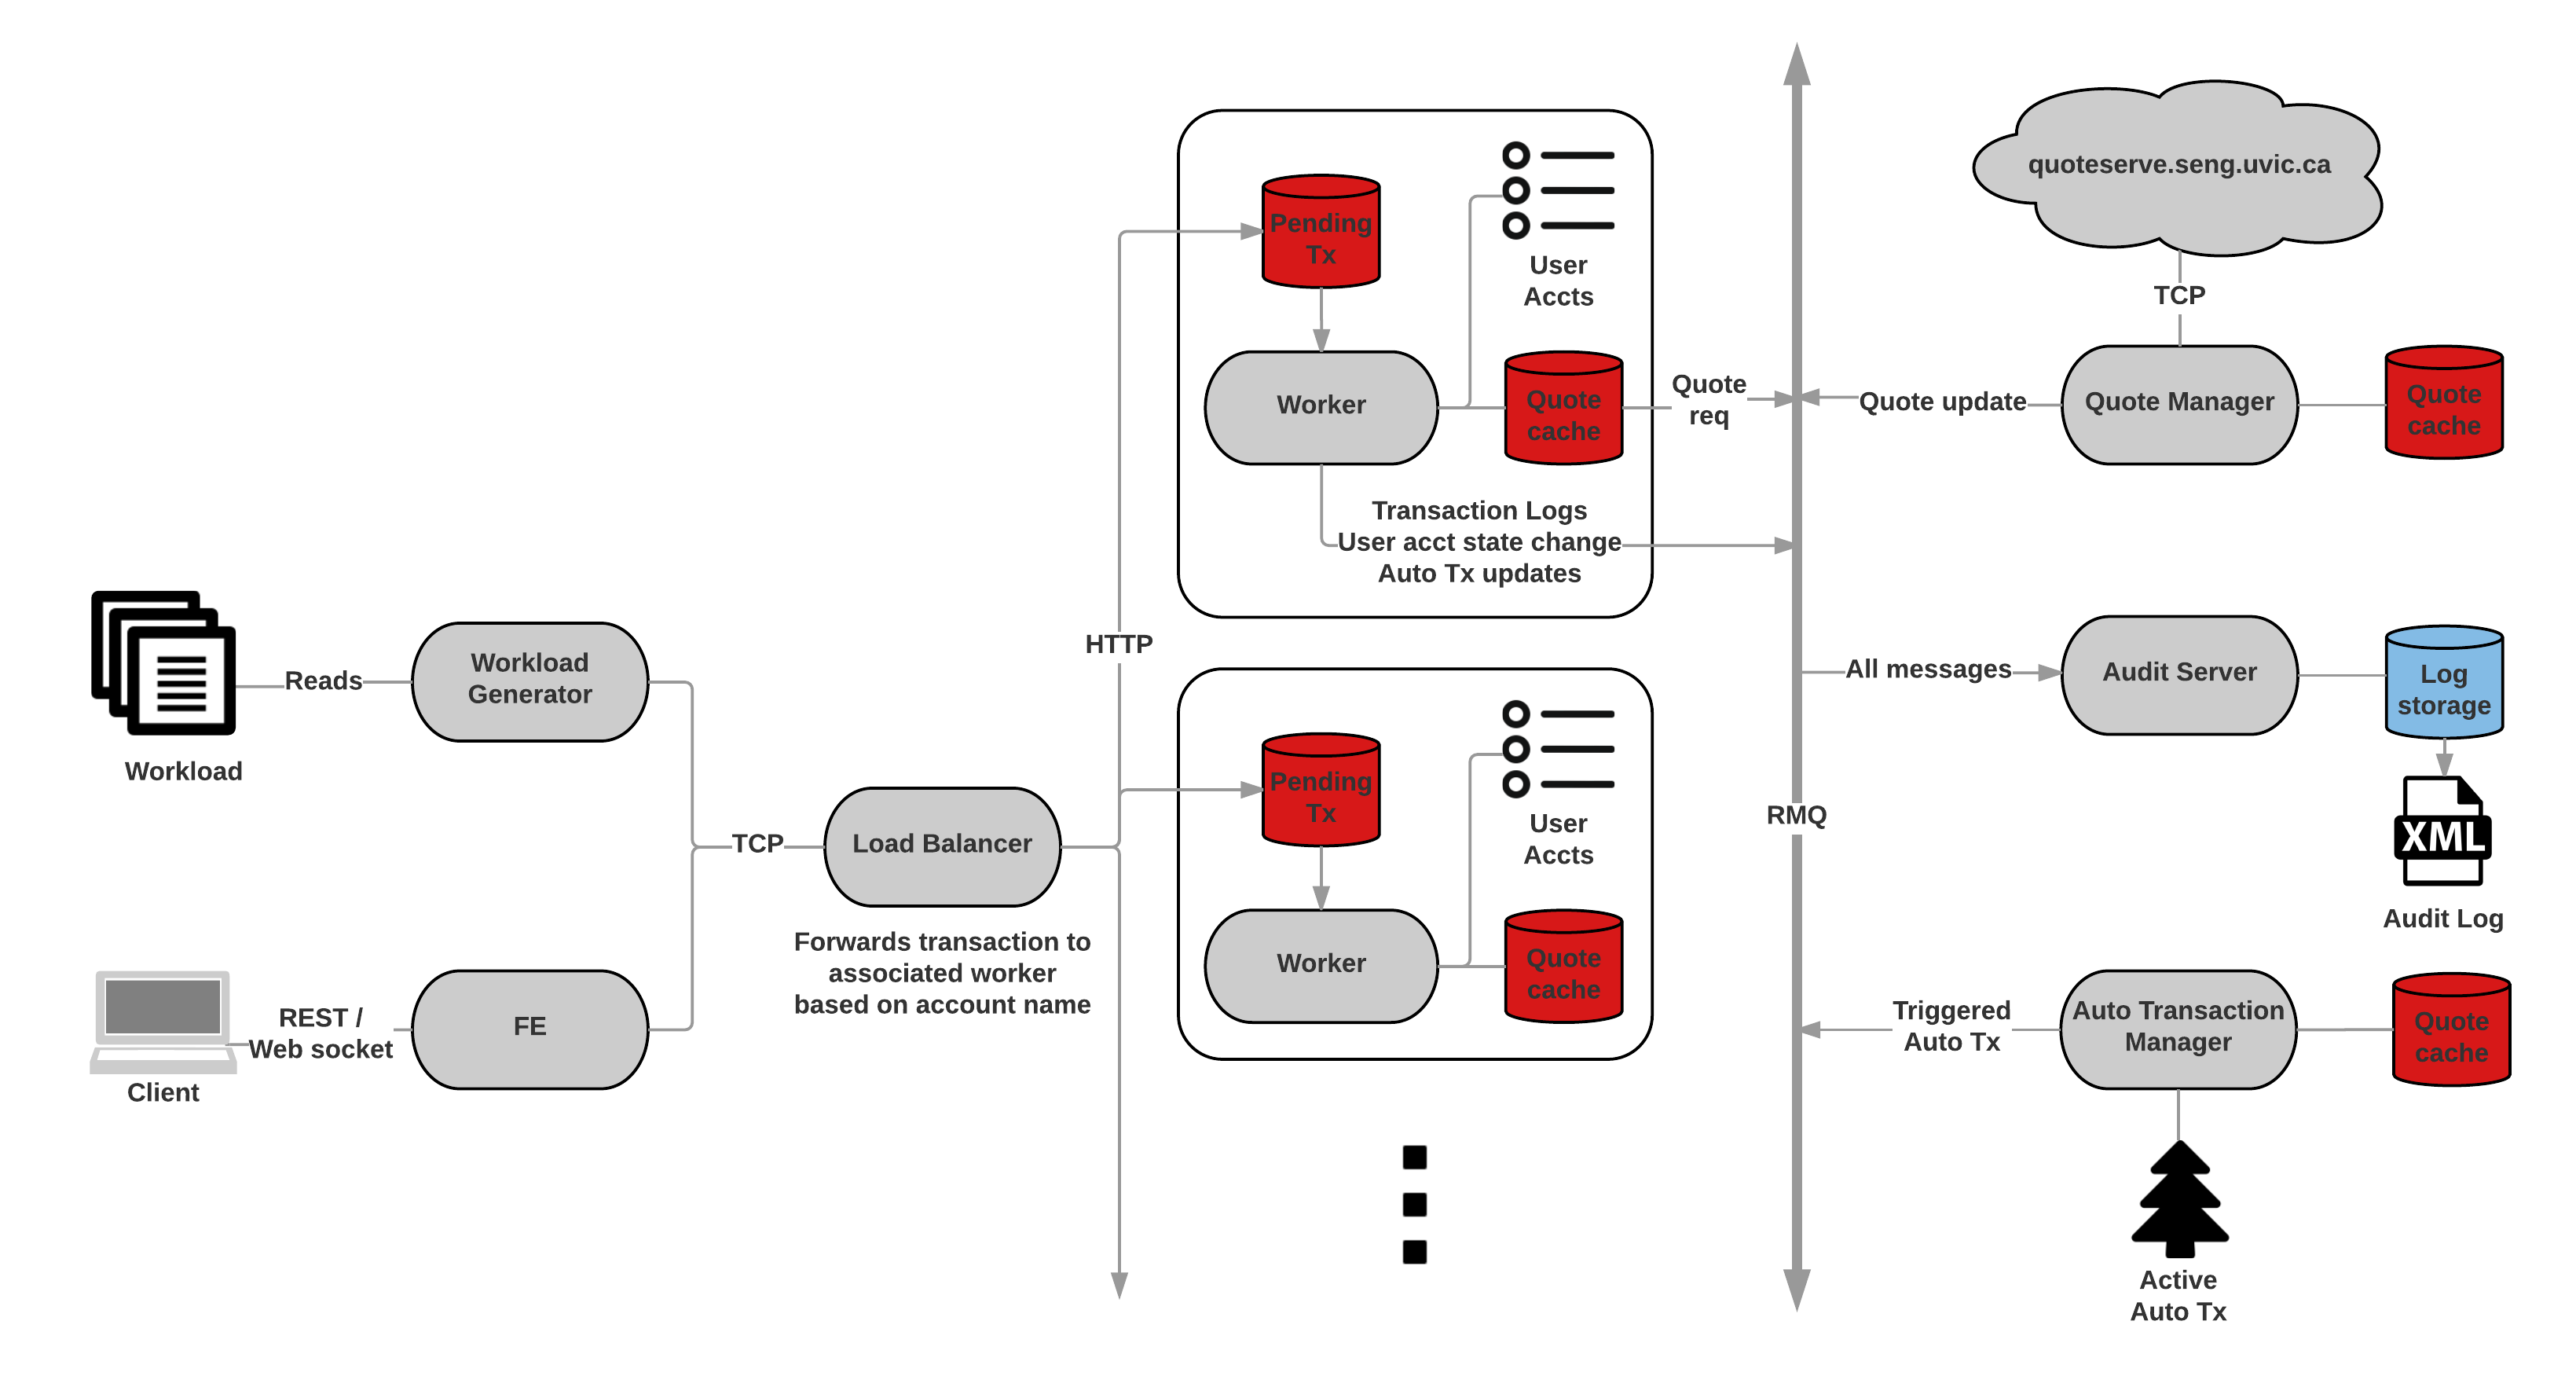
\includegraphics[width=0.85\linewidth]{graphics/arch-final}
  \caption[Final system architecture]{Final system architecture. Red databases are Redis caches, blue databases are Postgres.}
  \label{fig:arch-final}
\end{figure}

\subsection{Incoming traffic}
The method of load balancing had to be modified to account for serving of the frontend and connection of the websockets.
Request which enter the load balancer are given a session token, and are always routed back to the same worker.
This allows us to skip the microservice which would be responsible for serving an ACID database of userdata.
The root url serves an HTML page, which contains the login/create page if a user has not registered.
Once at this page, a user is able to register/login, at which point a socket connection will be made to the backend.
This socket connection will serve to asynchronously return the account state, as well as any output messages that need to be presented to the user.
We opted for an entirely event based pattern instead of trying to modify a request/response style page loading to fit the event system on the backend.
This allows all of our requests to be non blocking, and for the user to have the most up to date information all the time.

\subsection{Frontend}
The frontend consists of an authentication screen, and a loggedin view.
Each action results in a post request getting sent to the API.
Login maps to the \texttt{/login} API endpoint, create maps to the \texttt{/create} API endpoint, and all other actions map to the \texttt{/push} API endpoint.
Login and create are responsible for user authentication.
Once this is completed, the frontend also requests a consistent websocket connection over the \texttt{/ws} API endpoint.
This websocket connection is added to the socket hub on the backend.
Any time an event is completed on the backend, the socket hub returns the user’s socket connection and the event is fired over the socket to the users frontend.
Each response contains two portions of data: The updated user state, and a message to display on the output screen.
The updated user state is parsed on the frontend and displayed to the user.

\subsection{Worker}
The worker as a whole functioned relatively similar to the intended architecture.
It stores account data, a local quote cache, and is the workhorse of the entire distributed system.

\subsubsection{Account store}
Accounts are stored on the worker in memory.
Each worker is responsible for a sectioning of accounts.
Once a user has created an account on a worker, all of it’s incoming requests will be routed through that worker until the account is terminated.
While an in memory solution may not seem fault tolerant, all of the events are logged to an audit server, which can be used to replay events on another worker should the original worker crash or go down.
In the case of total system failure, the audit logger uses a persistent storage, Postgres, and the system could be brought online simply be replaying all of the transactions from when the audit logger was last live, to when it last went dark.

\subsubsection{Worker goroutines}
The worker ended up divided into seven goroutines.
Golang goroutines can be thought of simply as threads or processes which are time sliced.

\paragraph{\texttt{incomingTxWatcher}}
This was responsible for the http setup of the websocket handshaking, the frontend serving, as well as the \texttt{/push} API spinup.

\paragraph{\texttt{sendAutoTx}}
This goroutine spins up and pulls from two channels: \texttt{autoTxInitChan} and \texttt{autoTxCancelChan}.
When a user correctly produces an auto transaction by setting and amount and then a trigger value, it is pushed into the channel and pulled by this go routine.
In the case of an \texttt{autoTxInit}, we verify the local quote cache to determine if we can fire the trigger instantly, without the help of the autoTx manager.

If the trigger is valid already, it is fulfilled without leaving the worker.
If not, we simply publish it to the autoTx manager through its initialization autoTx RMQ.

\texttt{AutoTxCancel} works similarly, except any cancel requests are simply sent straight to the worker.
No trigger check is done, since there is no trigger check to do for a cancel.

\paragraph{\texttt{receiveAutoTx}}
This goroutine is the sister routine to \texttt{sendAutoTx}. \texttt{AutoTxFilled} types are sent back to the workers \texttt{autoTxQueue}, which is an RMQ direct exchange where the routing key is the worker ID.
When these filled requests come in, they contain an \texttt{AutoTxKey}, an \texttt{AddStock}, and an \texttt{AddFunds}.
The idea of this is that both buys and sells can be consumed on the same type, as the result of a buy is an amount of stock, and a remainder of cash, and the result of sell is an amount of stock (0) and a remainder of cash.
By unifying these two types, its possible to eliminate the forking behavior that would exist otherwise.

\paragraph{\texttt{catchQuoteBroadcasts}}
This goroutine is relatively simple, as it simply consumes from the quote broadcast exchange and caches the quote into the workers quote cache.

\paragraph{\texttt{fetchNewTx}}
This goroutine is responsible for consuming operations out of the the workers Redis queue and pushing them into the \texttt{unprocessedTx} channel, which is then pulled from by the \texttt{txWorker}.

\paragraph{\texttt{txWorker}}
This goroutine is responsible for the brunt of the processing which occurs on the worker.
Whenever an unprocessed transaction is pushed into the \texttt{unprocessedTx} channel, it is then processed by this worker.
The command is then parsed into a command object, which contains an execute function based on which type of transaction it is.
For example, add transactions will execute the add command in the backend.

\paragraph{\texttt{cleanAccountStore}}
Wakes every sixty seconds to remove expired buys and sells from all user accounts.
This prevents the memory loss associated with a user who initiates a large amount of buys or sells but never confirms those actions.

\subsection{Quote manager}
Quote updates involve every part of the distributed system and are the best demonstration of the efficiency of event-sourced architecture.
With event-sourcing, each service is free to define its own actions to events that occur in other parts of the system.
Figure~\ref{fig:arch-quotes} shows a typical quote request process.

\begin{figure}[tbph]
  \centering
  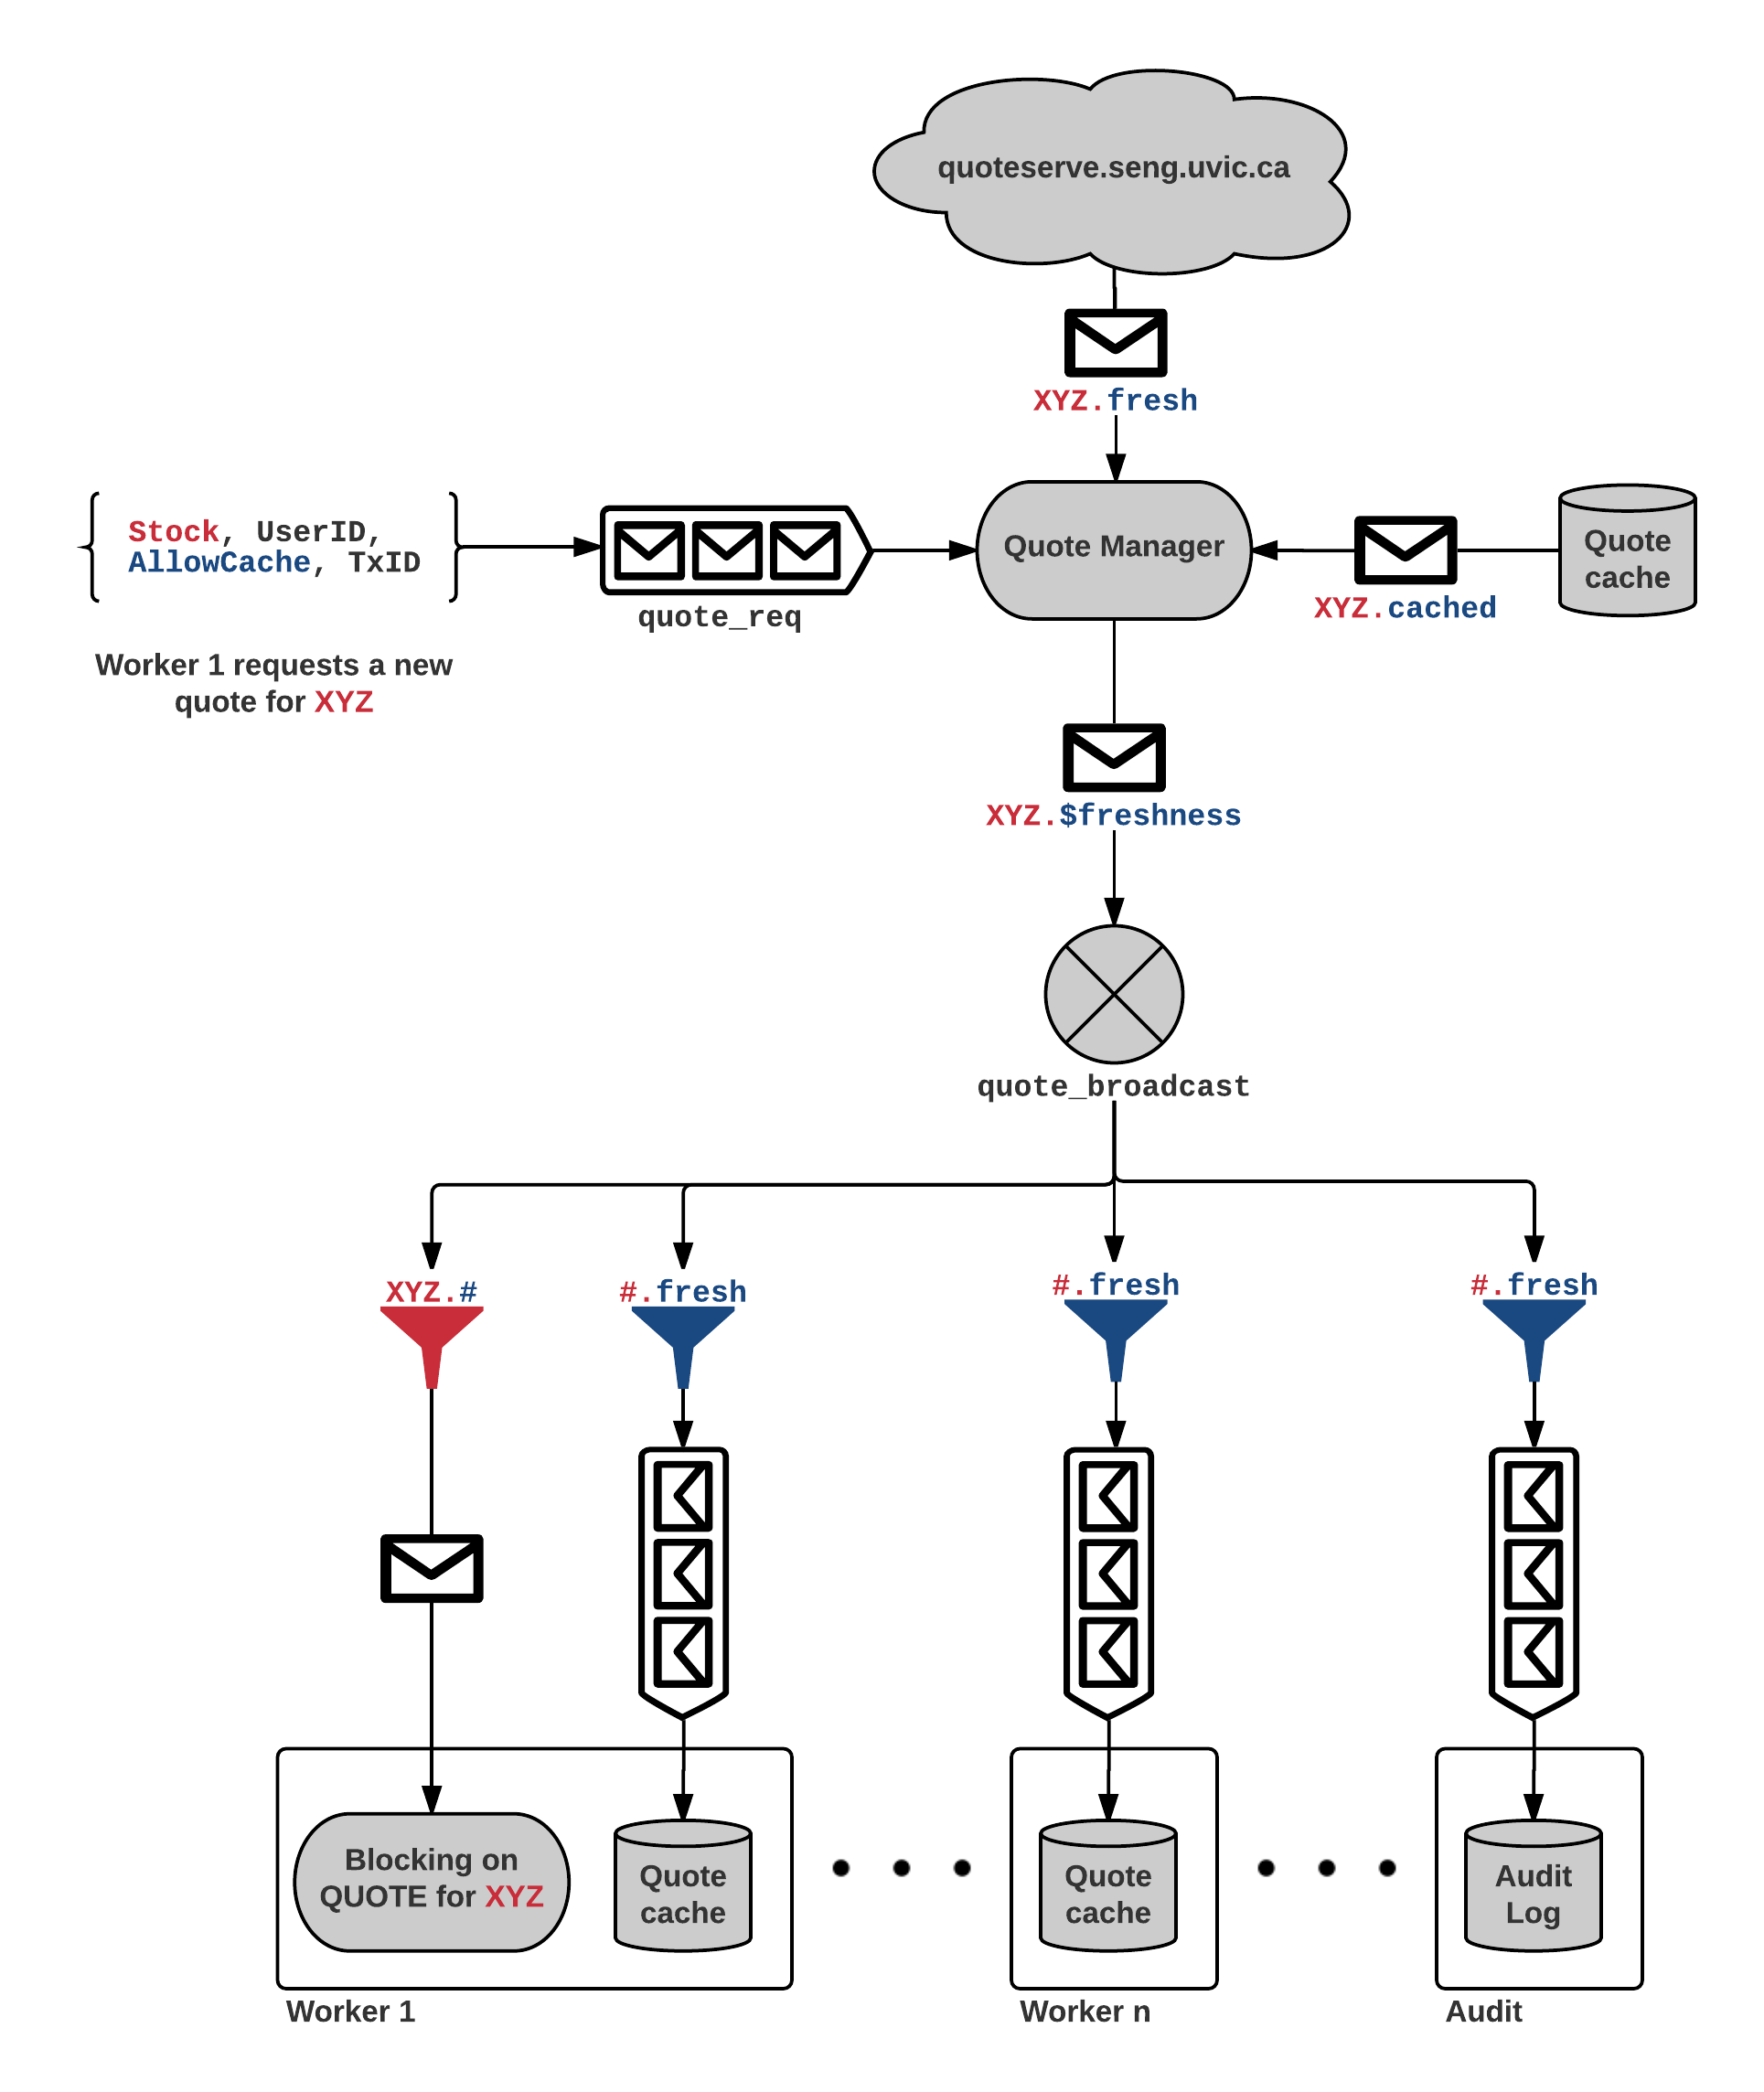
\includegraphics[width=0.85\linewidth]{graphics/arch-quotes}
  \caption{Service interactions for fulfilling a quote}
  \label{fig:arch-quotes}
\end{figure}

Workers generate requests for new quotes, specifying a stock and whether a cached response is allowed. (A \textsc{Buy} for a stock whose quote is about to expire can force a the retrieval of a fresh quote instead of passing the stale quote to the user.) The Quote manager pulls requests from \texttt{quote\_req} RMQ queue and checks for a cached value.
On a cache miss, or when forced by a worker, a new quote is requested from the legacy service using the timeout procedure detailed in~\ref{sec:timeout-effectiveness}.

Quotes are broadcast with a key consisting of the stock name and whether the quote was retrieved from a cache or from the legacy service (referred to as ``cached'' and ``fresh'' respectively).
Each part of the system filters broadcast messages for its particular purpose.
Workers and AutoTX managers need to maintain a local quote cache so they filter ``fresh'' quotes for cache updates.
The Audit Logger records quote requests for billing with the same filter.
The worker that generated the original request filters for the stock name.
This allows two workers to request and block on updates for the same quote and race their requests.
Both workers would resume execution when the first quote resolves.


\subsection{Audit logger}
The audit logger required significant redesign in order to accommodate high throughput logging.
Section~\ref{sec:log-buf} gives a thorough overview of the necessity of this design and its limitations.

\subsection{AutoTX manager}
The auto transaction manager was designed to be a central point where transactions could be confirmed and sent back to the respective workers. \texttt{AutoTxInit} messages are sent from the worker containing an \texttt{AutoTxKey} (\texttt{Stock}, \texttt{UserID}, \texttt{Action}) as well as an amount and a trigger. \texttt{AutoTxInit} objects are taken and inserted into an AutoTxStore, which contains a map of all \texttt{autoTxKeys} to \texttt{autoTxInits} (For cancellation of transactions), and a map of \texttt{TreeKeys} (\texttt{Stock}, \texttt{Action}) which maps a \texttt{Stock} and \texttt{Action} to a \texttt{Tree}.
When multiple auto transaction buys for a stock ABC comes in, they are inserted into a left leaning red black tree.
A red black tree was chosen because it excels at heavy read/write workloads and it is self balancing.
The auto transaction manager is responsible for requesting quote updates for each stock which resides in it’s store.

The auto transaction manager is also subscribed to the same quote broadcast exchange as the other workers.
When a new quote comes in, the buy and sell trees for that stock are observed.
It is very simple to partition the tree into fillable transactions and unfillable transactions, because red black trees are binary search trees and are balanced and ordered by their very nature.
For each fired trigger, the node is removed from both the tree and the map and then the \texttt{AutoTxFilled} transaction is sent back to the worker which instantiated it.

When \texttt{autoTxCancels} arrive at the autoTx manager, they are simply removed from the autoTx store.

While the auto transaction manager is the only place where user data meets, user data will never interact with any other user data, as comparisons are only done between the quote value and the amount specified by the user.
This ensures no cross contamination of data, or mismatching of auto transactions.



\chapter{Performance analysis}


\chapter{Performance analysis}

\section{User testing}
Validate command pre/post conditions. Tested through FE?

\chapter{Performance analysis}


\chapter{Performance analysis}

\section{Decreasing quote retrieval time}\label{sec:qs}

\subsection{Statistical analysis of legacy quote server}

\subsection{Using timeouts to ensure fast quote retrieval}

\subsection{Minimizing lingering TCP connections}

\subsection{Timeout effectiveness}
\section{Worker scaling}
Our domain decomposition recognizes that account actions are ``embarassingly parallel'' since accounts never interact with each other.
Scaling to accommodate more users is as straightforward as adding more workers.

\subsection{The sixty second golden window}
Many of the business logic requirements inherit time limitations from the sixty second validity window for a quote.
Therefore, if an entire workload can be completed in under sixty seconds then all quotes are valid for the entire run.
This gives rise to a ``golden window'' of performance where workloads that complete in within the window have drastically higher TPS than those that miss the window.

\begin{figure}[tbph]
  \centering
  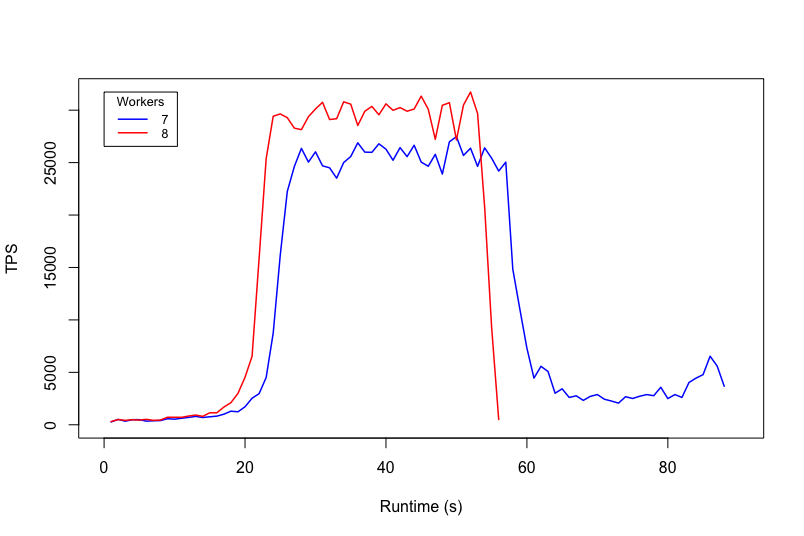
\includegraphics[width=0.7\linewidth]{../graphics/7v8}
  \caption[The golden window effect on TPS]{1000 user workload: 8 Workers, 18k average TPS; 7 Workers, 10k average TPS}
  \label{fig:tps-window}
\end{figure}

Even though approximately 90\% of the commands are completed in 60 seconds by seven workers in Figure~\ref{fig:tps-window}, the remaining 10\% need new quotes and the retrieval delay adds over 50\% to the total runtime.
The penalty for missing the golden window is severe.

\subsection{Scaling results}\label{sec:worker-scaling-results}
The 1000 user workload was used to test the effect of increasing the number of workers.
Figure~\ref{fig:tps-scaling} shows that increasing the number of workers decreases the total time to retrieve quotes, increases the maximum TPS and decreases the total runtime.

\begin{figure}[tbph]
  \centering
  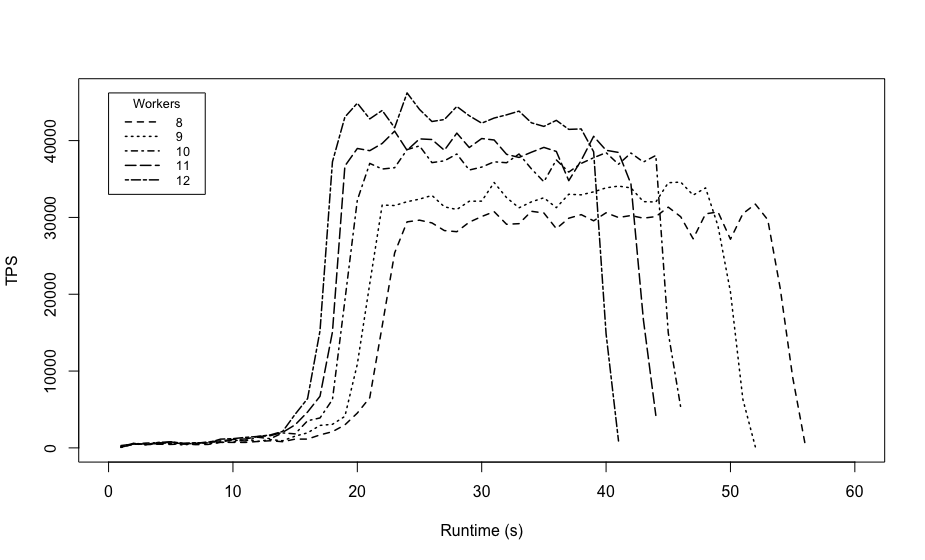
\includegraphics[width=0.8\linewidth]{../graphics/multi-worker}
  \caption{Scaling workers for 1000 user workload}
  \label{fig:tps-scaling}
\end{figure}

With twelve workers we achieved a maximum 26.1k average TPS for the 1000 user workload and a peak TPS over 45k. (See~\ref{sec:starvation} for why we did not add more workers.)

There are two distinct modes of operation for the system: quote-fetching and nominal\footnote{Specifically, the system is at ``nominal TPS'' when it is within 85\% of max TPS.} operation.
During quote-fetching, transactions in workers generate local quote cache misses and are blocked on responses from the quote manager.
During nominal operation the workers have a full set of quotes cached locally and no longer have to block on responses from network services.
The jaggedness in the nominal TPS region is noise from plotting a single run with each worker configuration.

The average TPS value during nominal operation indicates weak linear scaling with the number of workers.
Again, repeated runs should decrease the error.

\begin{figure}[tbph]
  \centering
  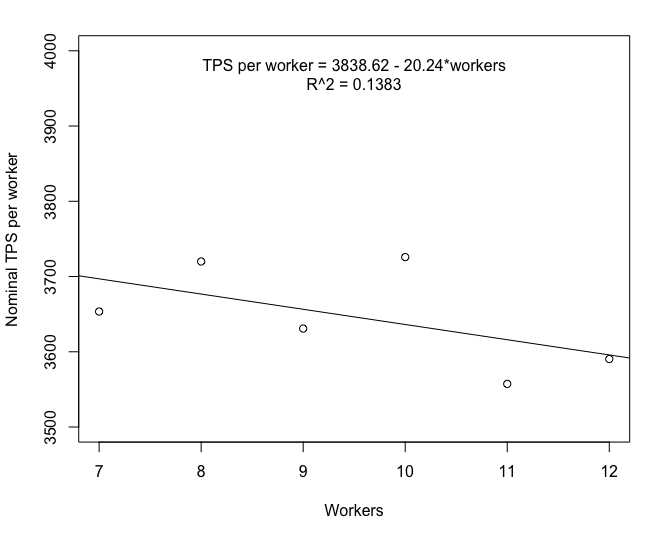
\includegraphics[width=0.7\linewidth]{graphics/tps-per-worker}
  \caption{TPS scaling with workers for 1000 user workload}
  \label{fig:tps-per-worker}
\end{figure}

It's important to note that even when runtime exceeds the golden window the nominal operation speed of the workers is relatively constant.
This indicates that successful methods for scaling the application will involve decreasing the time to reach nominal TPS and then adding more workers.
Chapter~\ref{ch:cap} documents our efforts to realize this scaling.


\section{Command execution time analysis}

\chapter{Performance analysis}

\section{Logging throughput}
The 1000 user workload was the first occasion for our system to operate at nominal TPS for a significant portion of its runtime\improvement{link to image with 100 v 1000 tps}.
Since each transaction needed to write at least one entry to the audit log the volume of log messages was unprecedented.
Controlling the ``firehose'' of log messages was the most significant architectural redesign.
It included several false starts and, ultimately, reached a workable but flawed solution.

\subsection{Limits of logging to a flat file}
From the initial prototype through the 100 user workload, the audit service wrote directly to an \texttt{.xml} file that could be submitted for validation.
Log messages were removed from RMQ and stored in memory for writing by separate threads.
However, running the 1000 user workload exceeded the rate that the audit service could clear messages from RMQ, causing a significant backlog of messages to develop.
As the total message backlog size approached 700k the rate that messages could be exchanged slowed, causing a slowdown in the rest of the system as execution was blocked on message exchange.
Soon after, services would fail as they lost their connection to the RMQ server.

As noted in the ``Production Checklist'' section of the RMQ user guide\footnote{\url{https://www.rabbitmq.com/production-checklist.html}}, performance is heavily tied to available RAM.
As the backlog increases RMQ will begin swapping RAM to disk to ensure persistence.
The IO penalty for writing to disk causes an intense slowdown.
Since the worker services generating the logs are not capable of throttling they eventually push RMQ into resource exhaustion and failure.

Direct to file logging was never intended for production use.
Creating per-user dumplogs would be onerous since there was no direct method for searching or sorting the log file.
Leaving the log file implementation in place for most of the project allowed us to focus development efforts on optimizing the quote manager and implementing the auto transaction service.
Letting RMQ fail illuminated the ``danger zone'' for RMQ on the lab machines.
Different audit logger refactors could be compared for effectiveness by monitoring the RMQ backlog.

\subsection{Logging directly to an RDBMS}\label{sec:log-rdbms}
The first refactor involved inserting logs into Postgres and writing to a file on an as-requested basis.
This solved the problem of creating per-user log files but throughput was significantly worse than writing direct to a file.
With direct to file, the 100 user workload with 100k transactions generated 2k backlogged messages on RMQ.
With the Postgres refactor, the 100 user workload resulted in a 20k message backlog.
No attempts at larger workloads were made after this poor result.

This performance slowdown is not surprising.
The flat file and RDBMS both store the pre-formatted \texttt{.xml} entry for the event.
In addition, the RDBMS stores extra data about the user name, transaction type and creation time to enable queries.
The RDBMS is storing more data than the flat file.
In addition, the RDBMS suffers a performance penalty from indexing data on insertion.
While there are methods to mitigate these problems, such as connection pooling, the performance degredation was extreme enough to justify larger service refactors.

\subsection{Processing logs with ELK}
An RDBMS enables rich querying and enforces data integrity \textemdash{} useful features that are not relevant for storing an append-only log.
Moreover, the indexing that provides those useful features introduces a performance penalty that limits throughput.
Specialized log storage solutions forgo rich indexing in order to maximize write throughput.

The Elasticsearch - Logstash - Kibana (ELK) suite of applications from elastic.co\footnote{\url{https://www.elastic.co}} is a popular distributed log storage method.
Logstash consumes and transforms data for indexing and storage in Elasticsearch.
Kibana is a graphical monitoring suite that provides information about the logging rate and health of the logstash and elasticsearch services.

A prototype was created that deployed the ELK stack in separate Docker containers collocated with the audit logger.
Logstash consumed messages directly from RMQ and sent them to Elasticsearch for indexing and storage.
The prototype had abysmal performance.
With the 45 user workload there was a 7k (out of 10k total) backlog.
Development was abandoned at this point.

The poor performance of the ELK stack was directly related to its resource limitations.
Each part of the ELK stack performs better with more available RAM.
Collocating all services severely limited the available RAM.
Also, ELK requires a non-trivial amount of JVM and OS tuning to provide optimal resource availability.
Although there are guides for this process it was unclear how to apply their recommendations on the tower of abstractions in the production environment: a docker OS on a VM OS on a host OS, each needing their own tuning.

The Elasticsearch scaling guide\footnote{\url{https://www.elastic.co/guide/en/elasticsearch/guide/current/scale.html}} recommends adding more shards (i.e. independent instances which maintain a partition of the data) to increase write throughput.
This throughput solution \textemdash{} a distributed system within a distributed system \textemdash{} directly links scaling to resource demand.
Scaling Elasticsearch would likely reduce the number of systems available to host workers and limit the maximum TPS.
The problem of high log throughput would be solved by removing the ability to create logs at a high rate.

\subsection{Buffered logging}\label{sec:log-buf}
The problem with the RDBMS solution in~\ref{sec:log-rdbms} is fundamentally a mismatch between the production and consumption rate of log messages.
The solution to this problem is to place a buffer between the producer and consumer.

\begin{figure}[tbph]
  \centering
  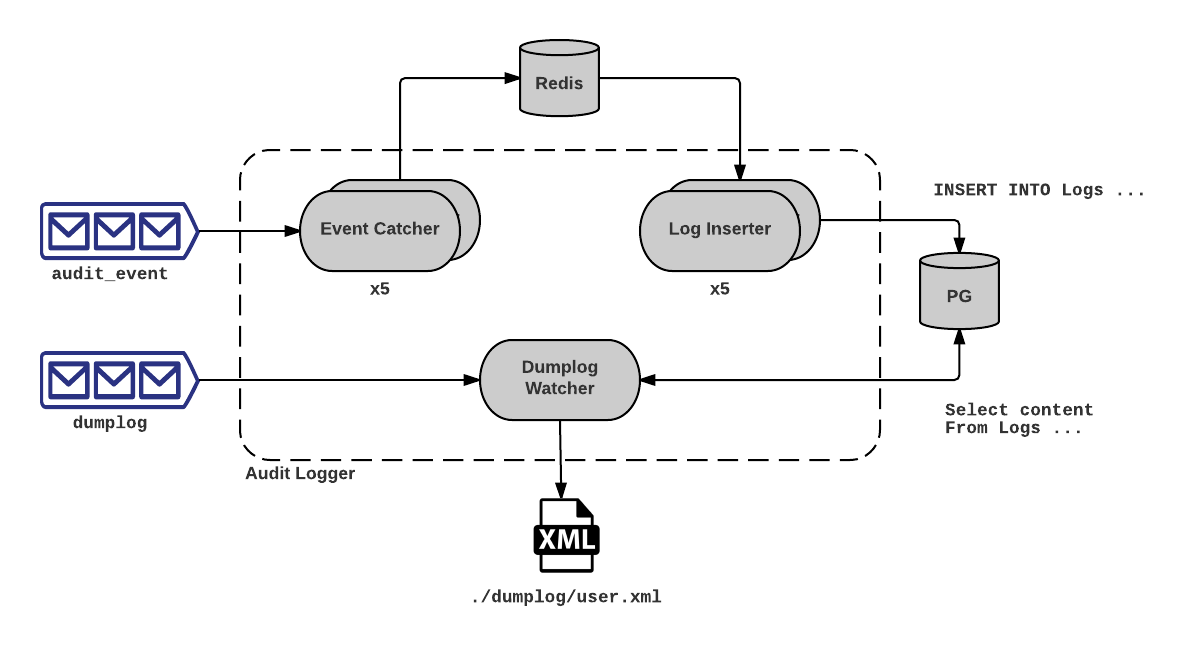
\includegraphics[width=0.95\linewidth]{graphics/audit}
  \caption{Buffered audit logger}
  \label{fig:audit}
\end{figure}

Figure~\ref{fig:audit} shows how multiple \texttt{Event Catcher} workers remove incoming log messages from RMQ and place them in Redis. \texttt{Log Inserter} workers remove items from Redis and store them in Postgres.
With this design, the 1000 user workload only reached a 20k backlog of messages and had no observed performance degradation.
Although a run would finish in around \SI{45}{\second} it would be upwards of \SI{6}{\minute} to finish insertion into Postgres.
When a message for a dumplog was processed it would display messages had successfully migrated to Postgres but was unaware of those still in Redis.
This is a soft violation of the business requirement that a dumplog should show all transactions preceeding itself.
We believe this is acceptable since, in actual use, there is no clear ``end of work'' to capture.
All log messages will make it in to Postgres for querying so the requirent is \textit{eventually} satisfied.

This method has an upper limit to its effectiveness since the Redis buffer could run out of storage space under periods of sustained high TPS.
The boundary of the buffer memory was not encountered during any testing and we cannot speculate about its value.
In order to determine the limits we would need a workload file larger than the final workload.
Alternatively, we could induce a period of sustained high TPS by removing the requirement to re-fetch expired quotes and concatenate existing workloads.

\subsection{Alternate solutions}
When the buffer method in~\ref{sec:log-buf} reaches its limit there are several possible development paths for proceeding forward:

\begin{enumerate}
  \item \textbf{Agglomerate messages}: Message traffic can be reduced by combining multiple log events into one message.
Workers would only emit messages for logging at fixed intervals or after a certain number of events (whichever comes first) and reduce the overhead associated with creating, sending and processing RMQ messages.
The optimal message size would have to be determined through experiment.
  \item \textbf{RMQ scaling}: RMQ is capable of its own distributed deployment.
Increasing resources available to the message bus would allow more messages to be stored before removal into the buffer.
  \item \textbf{Robust message passing}: Apache's Kafka\footnote{\url{https://kafka.apache.org}} provides functionality similar to RMQ but is optimized for message storage and large backlogs.
This allows consumers to operate at different rates and removes the need to process log messages faster.
\end{enumerate}

\section{Quote manager scaling}
The system's TPS grows almost $10\times$ once a full set of quotes has been retrieved.
Further increases to average TPS could be gained by decreasing the time spent fetching quotes.
The methods in~\ref{sec:qs} brought the quote server response time to its lower limit so further efficiency could only come from horizontally scaling the quote managers.
Intuitively, doubling the number of quote managers should decrease the total time to retrieve all quotes by half, provided the workload is split evenly.
If only it were so simple.

\subsection{Building a ``snoopy'' quote manager}
With one week until the final deadline we decided to refactor the quote manager to participate in a multi-quote manager environment.
We ported the ``snoopy caching'' functionality from the worker and audit logger into the quote manager.
The ``snoopy'' quote server could listen to quote broadcasts and update its local cache accordingly.
With this functionality, multiple quote managers could act as workers servicing requests from a single RMQ queue. 

A message header with the ID of the quote manager that serviced the request was added to all quote broadcasts.
The quote manager cache updaters would discard messages that originated from its own quote manager.
This is inefficient but necessary because RMQ does not allow an ``anti-match'' for message routing keys.
That is, one cannot specify, "Capture all messages \textit{except} ones that follow this pattern.''

Total development effort was approximately one hour.

\subsection{Performance analysis}
Figure~\ref{fig:snoopy-qs} shows that TPS correlates \textit{negatively} with the number of snoopy quote managers.
This is very counter-intuitive and deserves reflection.

\begin{figure}[tbph]
  \centering
  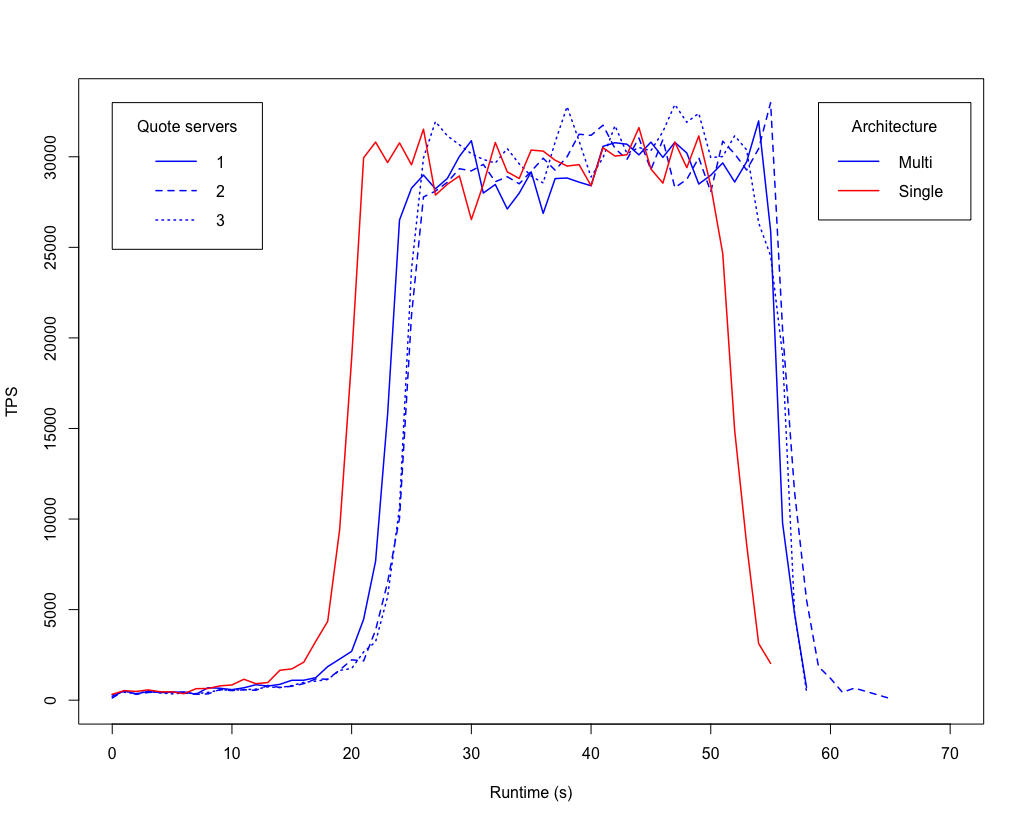
\includegraphics[width=0.85\linewidth]{../../data/tps/multi_vs_single_qs}
  \caption[Snoopy quote manager performance]{Performance of multi and single quote manager designs on 1000 user workload}
  \label{fig:snoopy-qs}
\end{figure}

Comparing the single quote manager deployment in multi and single architectures gives a sense of the overhead associated with discarding quote broadcasts.
The relation becomes less clear when two and three quote managers are used: the system benefits from having to retrieve fewer quotes per quote manager but adding quotes to the cache also has a delay.
The benefits from horizontal scaling start to manifest when three quote managers are used, but it takes the form of, ``things stopped getting worse,'' instead of ``performed better than a single quote manager.''

The single architecture quote manager is very fast because it already functions like a multi machine quote manager.
Each new request spawns a thread that handles communication with the legacy service.
Most of the threads are blocking on a response from the legacy service making it very likely that a new thread will find the application in an idle state.
Since workers block on the completion of a quote command the maximum number of simultaneous quote requests is equal to the number of workers.
Hence, the number of threads requesting quotes in the quote manager is capped, thus preventing thread creation runaways and CPU starvation in the quote manager.
Adding more quote managers doesn't increase the number of simultaneous quotes that can be requested by workers.

\subsection{Alternate solutions}
The snoopy quote manager was implemented because it was a small amount of development effort for a large potential payoff.
There is another way to implement multiple quote managers, although it is more complicated: quote symbols could be hashed to associate with unique quote managers.
This prevents the need for quote managers to do snoopy caching.
However, it introduces problems with scaling since the hash will depend on the number of available quote managers.

The snoopy quote manager can scale easier since failures would be independent.
As the number of workers continues to grow, Figure~\ref{fig:snoopy-qs} should be re-run to determine the break point between the communication overhead and the increased capacity for simultaneous quote requests.


\section{Worker loading}
To run the workload files we loaded sections of 3300 transactions into workers in a round-robin manner.
By measuring the total number of transaction in a worker's backlog at each loading cycle we could determine the limits of our round-robin loading method.

\subsection{Worker backlog analysis}

\begin{figure}[tbph]
  \centering
  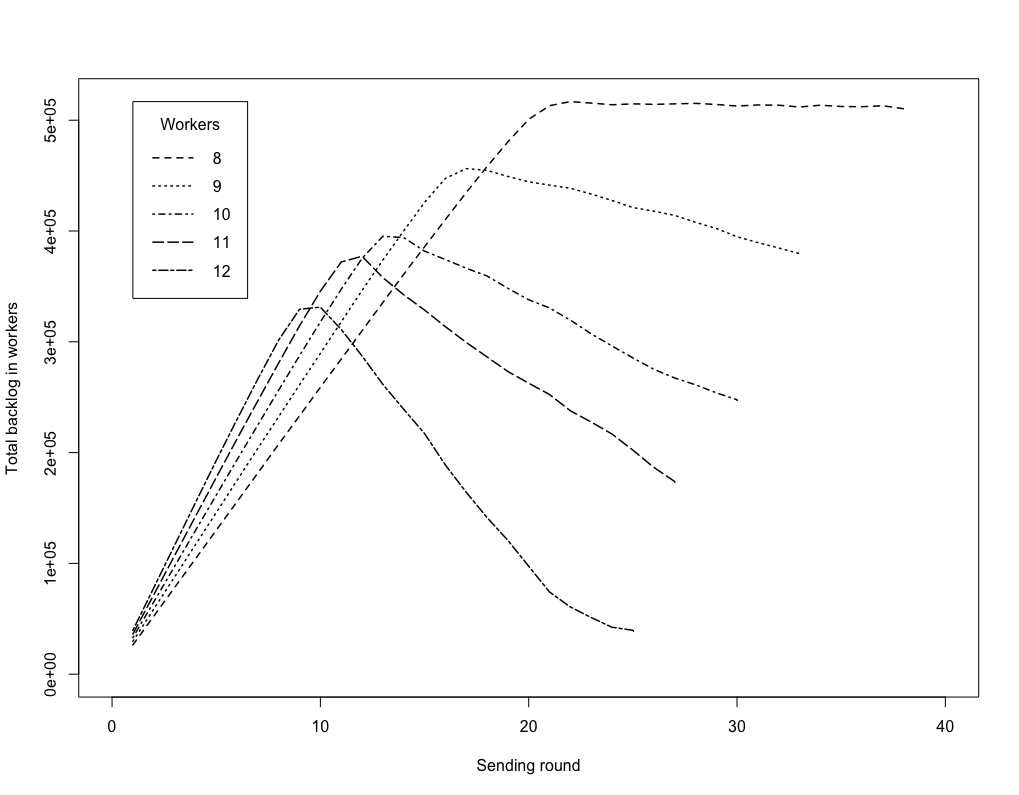
\includegraphics[width=0.9\linewidth]{graphics/backlog_by_workers}
  \caption{Total worker backlog for 1000 user workload}
  \label{fig:backlog-total}
\end{figure}

The curves in Figure~\ref{fig:backlog-total} have two distinct parts: an upward slope that becomes steeper as the number of workers before coming to a maximum and either plateauing, as with eight workers; decreasing at a fixed rate, as with nine to eleven workers, or; decreasing and leveling out, as with twelve workers.
It's important to note that the x-axis represents loading cycles and not a uniform time scale.
Round robin loading cycle times increase as the number of workers increases.

The slope of the curve represents the ratio of transactions coming in to a worker over transactions completed between successive cycles.
Essentially, this is
\begin{equation*}
  {\SI{3300}{transactions per cycle} \times \si{cycles per second} \over \si{transactions per second}}
\end{equation*}
The peak in the curves occurs when the system has retrieved a full load of quotes the transactions per second increases drastically.
For eight workers, the slope is approximately 1, indicating that the input and output rates are equal.
The work in~\ref{sec:worker-scaling-results} indicates that the transaction input rate must be approximately \SI{3600}{transactions per second} for each worker.
As the number of workers increases, the number of transactions per second for a worker stays (mostly) constant but the cycles per second decreases.
The leveling off with twelve workers indicates that the workers are starved for transactions near the end of the run.

The change in the rising slopes is also affected by the increased cycle time but the correlation is less direct.
During loading, the transactions per second is significantly lower than 3300 and constant regardless of the number of workers.
The slope increases with the number of workers because the capacity for transactions in the system increases (i.e. each worker has its own cache).
As the cycle times become longer this decreases the slope.

\subsection{Worker starvation analysis}\label{sec:starvation}

\begin{figure}[tbph]
  \centering
  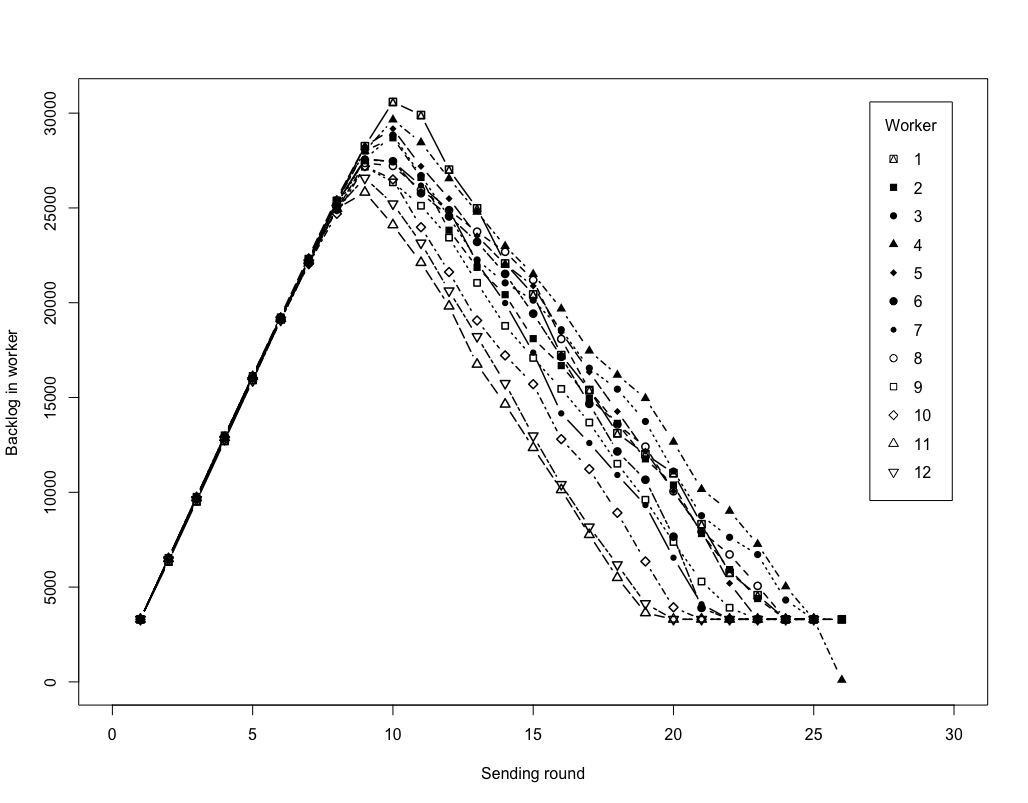
\includegraphics[width=0.85\linewidth]{../../data/worker-load/backlog_12w}
  \caption{Workers entering starvation during a 1000 user workload}
  \label{fig:backlog12w}
\end{figure}

Figure~\ref{fig:backlog12w} shows how workers entering starvation at different times.
All workers have identical backlogs up until the peak where higher-numbered workers operate at nominal TPS earlier.
This is because the low-numbered workers early in the round-robin cycle are ``alone'' for longer with the transaction list and are more likely to encounter uncached quotes.
High-numbered workers benefit from the pre-caching.
Unfortunately, they enter starvation approximately ten cycles before loading finishes and represent an inefficient use of resources.

The rates of descent are mostly uniform, with the exception of worker 4 (machine B133).
Consistently, this machine performed worse than its peers.
This could be the result of hardware aging and general, spooky ``cruft'' on the machine or a non-uniformity in the workload distribution.
The latter is unlikely since worker 4 was slow regardless of the total number of workers.

We did not undertake any tests with thirteen workers because of these results with twelve \textemdash{} adding more workers would cause the system to enter starvation earlier and would be a poor use of resources.

\subsection{Alternate solutions}
The ideal operating state is when the incoming and outgoing transaction rates are equal.
In order to achieve this state we would have to implement a feedback system with the transaction loader.
The number of backlogged transactions in a worker could change the number of transactions sent in a loading cycle.

Though not trivial, this is a very tractable solution.
However, we feel it would be overly specific to the testing environment.
Could an actually existing trading system exert backpressure on user loads to throttle demand? This seems unlikely, or at least one that would lead to frustrated users.
Further testing should involve a dynamic \textit{stream} of transactions that could exhibit richer behavior like cyclic demand cycles and surges.
Though the same risk of overfitting the prototype software to the test environment is present, the fidelity has increased and the solutions should be more generally applicable.
 

%%%%%%%%%%%%%%%%%%%%%%%
% 	  Referrences
%%%%%%%%%%%%%%%%%%%%%%%
\newpage
\renewcommand*{\UrlFont}{\rmfamily} % preserve default font for URLs
\printbibliography[heading=bibintoc,title={References}]

%%%%%%%%%%%%%%%%%%%%%%%
% 	  Back Matter
%%%%%%%%%%%%%%%%%%%%%%%

\StartAppendices{}
\section{Command execution time analysis}

\end{document}
